\usepackage{}\documentclass[a4paper, 12pt]{article}
%\input{numeric.bbx}
\usepackage[portuguese]{babel}
\usepackage[utf8]{inputenc}
\usepackage{amssymb}
\usepackage[table]{xcolor}%https://tex.stackexchange.com/questions/50349/color-only-a-cell-of-a-table/50351
\usepackage{amsmath}
\usepackage{colortbl}
\usepackage{tocloft}
\usepackage{indentfirst}
\usepackage{graphicx}
\usepackage{graphics}
\usepackage{float}
\usepackage{placeins}
\usepackage{siunitx}
\usepackage{tabularx}
\usepackage{color}
\usepackage[pdftex]{hyperref}
%\usepackage[alf]{abntex2cite}
\usepackage[colorinlistoftodos]{todonotes}
\usepackage[nottoc]{tocbibind}
\usepackage[sort,numbers]{natbib}
%\usepackage{cite}
\usepackage{biblatex} %Imports biblatex package
\addbibresource{sample.bib} %Import the bibliography file
\usepackage[framed,numbered,autolinebreaks,useliterate]{file}
\usepackage{listings}
\usepackage{color} %red, green, blue, yellow, cyan, magenta, black, white
\definecolor{mygreen}{RGB}{28,172,0} % color values Red, Green, Blue
\definecolor{mylilas}{RGB}{170,55,241}


 \definecolor{Blue}{rgb}{0,0,0.9}
%\title{Trabalho 1 - ENG1420}

%author{Paloma Sette \\ Vivian Suzano}

%\date{\today}

\begin{document}
%\maketitle

\begin{titlepage}
	\begin{center}
		

\vspace{10pt}
%\begin{figure}[!ht]
%\centering
%
\includegraphics{puc-rio-logo.png}

%\end{figure}
\begin{figure}[!ht]
\centering

\includegraphics{images/puc-rio-logo.png}
\end{figure}
\huge{Laboratório de Controles e Servomecanismos}
        \vspace{70pt}
        
		\textbf{ENG1418}
		\textbf{\large{\\Trabalho 1}}
		\textbf{\large{\\Sensores}}
		\vspace{65pt}
		
	\end{center}
	
	\begin{flushleft}
		\begin{tabbing}
			Alunos\qquad\qquad\=\>Gabriel Mota Botelho - 1620628\\
			\>Paloma Fernanda Loureiro Sette - 1621595\\
			
			Professor(a)\>Vivian Suzano Medeiros\\
	\end{tabbing}
		  
	\end{flushleft}
	\begin{center}
		%\vspace{\fill}
		Rio de Janeiro, 24 de Março de 2022
	\end{center}
\end{titlepage}
%%%%%%%%%%%%%%%%%%%%%%%%%%%%%%%%%%%%%%%%%%%%%%%%%%%%%%%%%%%
\newpage
\tableofcontents
\thispagestyle{empty}

\newpage
\pagenumbering{arabic}

\newpage

%\newcommand{\listequationsname}{Lista de Equações}
%\newlistof{myequations}{equ}{\listequationsname}
%\newcommand{\myequations}[1]{%
%\addcontentsline{equ}{myequations}{\protect\numberline{\theequation}#1}\par}

%\listofmyequations
\newpage


\newpage

\listoffigures
\thispagestyle{empty}

\newpage
%%%%%%%%%%%%%%%%%%%%%%%%%%%%%%%%%%%%%%%%%%%%%%%%%%%%%%%%%
%%%%%%%%%%%%%%%%%%%%%%%%%%%%%%%%%%%%%%%%%%%%%%%%%%%equ
\section{Introdução}
Esta pesquisa consiste no primeiro trabalho da disciplina de Laboratório de Controles e Servomecanismos, onde realizamos uma breve abordagem acerca de Transdutores e apresentamos um tipo analógico (\textit{Pressure Trabsducter}) e um digital (\textit{Encoder}) como exemplo. Após, abordamos sobre os Sensores de som e os sensores infravermelho com a finalidade de medição de distância, conforme designado.

\section{Transdutores}
Um transdutor detecta uma grande variedade de diferentes formas de energia, tais como movimento, sinais elétricos, radiação, energia magnética etc.
\paragraph{}O transdutor converte a informação de uma determinada grandeza física para um sinal elétrico. É um dispositivo eletrônico que possui duas funções principais, isto é, sensoriamento e transdução. Neste primeiro, ele detecta uma quantidade física e, por meio deste segundo, realiza a transdução para trabalhos mecânicos ou sinais elétricos.
\paragraph{}Há diversos tipos de sensores e transdutores, que são classificados pelos critérios a seguir:
\begin{itemize}
    \item  Por transdução passiva e ativa;
    \item Como transdutor primário e secundário;
    \item Como transdutor analógico e digital;
    \item Como transdutor inverso.
\paragraph{} O diagrama abaixo denota alguns exemplos.    

\begin{figure}[H]
\centering
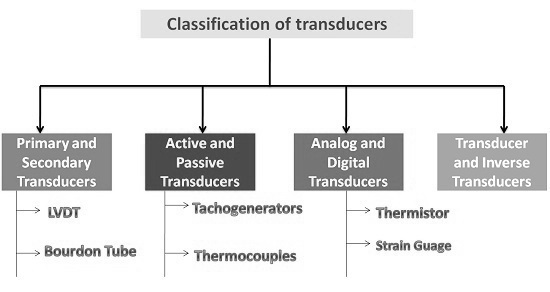
\includegraphics[scale = 0.4]{images/Transducer-types.jpg}
\label{filtro1}
\caption{Diagrama demonstrativo dos tipos de transdutores (Fonte: Test And Measurement World - https://www.test-and-measurement-world.com/Terminology/Analog-Transducer-vs-Digital-Transducer.html)}
\end{figure}
\end{itemize}

\newpage
% ... some material
\afterpage{%
\usepackage[utf8]{inputenc}
\usepackage{geometry}
    \newgeometry{left=2cm,right=1.5cm,top=1.5cm,bottom=1.5cm}


} % end of \afterpage{...} material
% ... still more material
\paragraph{} Estamos especialmente interessados em abordar a respeito dos transdutores analógicos e digitais. Para isso, selecionamos dois instrumentos específicos: Transdutor de Pressão (analógico) e Encoder (digital)

\subsection{Sinais Analógicos x Digitais}

\subsubsection{Características do Sinal Analógico}
\begin{itemize}
    \item O sinal trafega por uma faixa de frequência muito grande, o que resulta em um grande número de oscilações .
    \item Pode ser periódico ou não periódico.
    \item O sinal analógico funciona em dados contínuos.
    \item A curva da onda senoidal apresenta intervalos que variam entre 0 e 10, sendo esta uma das características mais decisivas deste formato. Isso porque o sinal analógico passa por todos os infinitos valores existentes entre estes dois extremos (1.56, 3.586, 9.814...).
    \item O formato de saída do sinal analógico é como Curva, Linha ou Gráfico, portanto, pode não ser significativo para todos.
\end{itemize}

\begin{figure}[H]
\centering
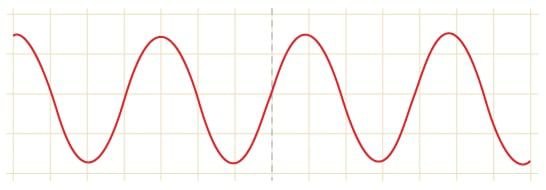
\includegraphics[scale = 0.5]{images/i295918.jpeg}
\label{filtro1}
\caption{Sinal analógico senoidal (Fonte: Canal Tech)}
\end{figure}

\restoregeometry

\newpage
\subsubsection{Características do Sinal Digital}
\begin{itemize}
    \item  Apresenta apenas valores discretos no tempo e na amplitude.
    \item Este tipo de sinal eletrônico pode ser processado e transmitido melhor em comparação com o sinal analógico.
    \item Os sinais digitais são versáteis, por isso são amplamente utilizados.
    \item mais precisão, menos custos e menos tempo de processamento.

\end{itemize}

\begin{figure}[H]
\centering
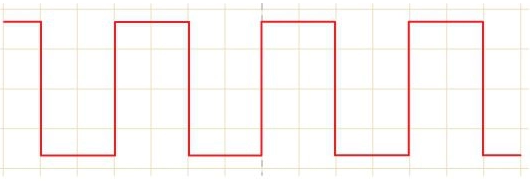
\includegraphics[scale = 0.5]{images/dig-signal.png}
\label{filtro1}
\caption{Sinal digital - onda quadrada (Fonte: Canal Tech)}
\end{figure}

\paragraph{ É interessante enfatizarmos as principais diferenças entre sinais analógicos e sinais digitais:}

\begin{itemize}
    \item  Um sinal analógico é um sinal contínuo, enquanto os sinais digitais são sinais separados no tempo.
    \item O sinal analógico é denotado por ondas senoidais enquanto o sinal digital é denotado por ondas quadradas.
    \item O sinal analógico usa uma faixa contínua de valores que ajudam a representar informações, por outro lado, o sinal digital usa 0 e 1 discretos para representar informações.
    \item Comparando sinais digitais versus analógicos, a largura de banda do sinal analógico é baixa, enquanto a largura de banda do sinal digital é alta.
    \item Os instrumentos analógicos fornecem erros observacionais consideráveis, enquanto os instrumentos digitais não causam nenhum tipo de erro observacional.
    \item O hardware analógico não oferece implementação flexível, mas o hardware digital oferece flexibilidade na implementação.
    \item Comparando o sinal analógico com o digital, os sinais analógicos são adequados para transmissão de áudio e vídeo, enquanto os sinais digitais são adequados para computação e eletrônica digital.

\end{itemize}



\subsection{Transdutor de pressão}
\subsubsection{Princípio de funcionamento}
É necessario que compreendamos o funcionamento do sensor de pressão e do efeito piezoresistivo, que é medido pelo medidor de tensão (às vezes chamado de \textit{strain gage}). Um \textit{strain gage} de folha de metal é um transdutor cuja resistência elétrica varia com a pressão aplicada. Em outras palavras, ele converte força, pressão, tensão, compressão, torque e peso (também conhecidos como sensores de peso) em uma mudança na resistência elétrica, que pode ser medida.

\textit{Strain gauges} são condutores elétricos firmemente presos a um filme em forma de ziguezague. Quando este filme é puxado, ele – e os condutores – estica e alonga. Quando é empurrado, ele se contrai e fica mais curto. Essa mudança na forma faz com que a resistência nos condutores elétricos também mude. A deformação aplicada no transdutor de pressão pode ser determinada com base neste princípio, pois a resistência do medidor de tensão aumenta com a deformação aplicada e diminui com a contração.

\begin{figure}[H]
\centering
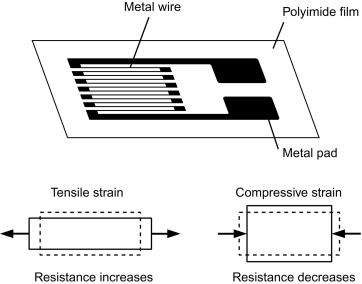
\includegraphics[scale = 0.8]{images/METAL-FOIL-STRAIN-GAUGE-LOAD-CELL.PNG}
\label{filtro1}
\caption{Strain Gage de folha de metal (Fonte: ScienceDirect)}
\end{figure}

Um Transdutor de Pressão, muitas vezes chamado de Transmissor de Pressão, é um instrumento que converte um sinal pneumático para um sinal elétrico analógico. 
\paragraph{}Um dos transdutores de pressão mais comuns é o que possui base de sensor deformação/tensão. Ao receber um sinal pneumático, ocorre uma deformação física dos sensores ligados ao diafragma do instrumento. Estes sensores estão ligados por uma configuração de ponte de \textit{Wheatstone}. Isso significa que quatro extensômetros são interconectados como um circuito de loop e a grade de medição da pressão que está sendo medida é alinhada de acordo.

\paragraph{}A pressão que chega ao transdutor produz uma deflexão no diafragma, ocasionando a deformação dos sensores que, por sua vez, irá produzir uma alteração de resistência elétrica proporcional à pressão aplicada. Assim, um sinal analógico correspondente é transmitido.

\subsubsection{Saída Elétrica}
Os Transdutores de Pressão normalmente estão disponíveis com três tipos de saída elétrica: \textit{milivolt} (mV), tensão amplificada e 4-20 mA.


Podemos citar, como exemplo, os sensores de pressão industriais FUTEK. Eles utilizam o efeito piezoresistivo, que consiste em extensômetros de folha de metal montados em um diafragma. À medida que a pressão muda, o diafragma muda de forma, fazendo com que a resistência nos extensômetros mude, permitindo que as mudanças de pressão sejam medidas eletricamente. Essses sensores de pressão produzem naturalmente um sinal elétrico em milivolts que varia proporcionalmente com a pressão e a tensão de excitação do sensor (mV/V). 

Os amplificadores de ponte de medidor de tensão fornecem tensão de excitação regulada e convertem o sinal de saída mv/V em outra forma de sinal que é mais útil para o usuário. O sinal gerado pela ponte do strain gage é um sinal de baixa intensidade e pode não funcionar com outros componentes do sistema, como PLC, módulos de aquisição de dados (DAQ) ou computadores. Assim, as funções do condicionador de sinal do sensor de pressão incluem tensão de excitação, filtragem ou atenuação de ruído, amplificação de sinal e conversão de sinal de saída.



\subsubsection{Exemplos de aplicação}
\paragraph{1. Monitoramento dos fluxos do processo:}


Sensores de pressão diferencial são usados extensivamente em fluxos de processo onde um fluido precisa passar por algum tipo de barreira, como um filtro. Em condições normais, a diferença de pressão entre a pressão a montante (frequentemente chamada de pressão de linha ou afluente) e a pressão a jusante (efluente) deve ser nula ou mínima. À medida que o filtro fica bloqueado com contaminantes, a pressão a jusante diminuirá, o que faz com que a diferença medida aumente.

A saída do sensor pode ser calibrada para mostrar a diferença de pressão máxima permitida em escala total. Por exemplo, uma saída de 4-20mA pode ser calibrada para mostrar 20mA quando a diferença de pressão atingir o máximo permitido, mas ler 4mA quando a diferença de pressão for nula.

Os sensores de pressão diferencial medem a diferença entre as pressões de afluente e efluente de um filtro, por exemplo, que deve ser nula em condições normais de operação, mas aumentará à medida que o filtro ficar entupido.

\begin{figure}[H]
\centering
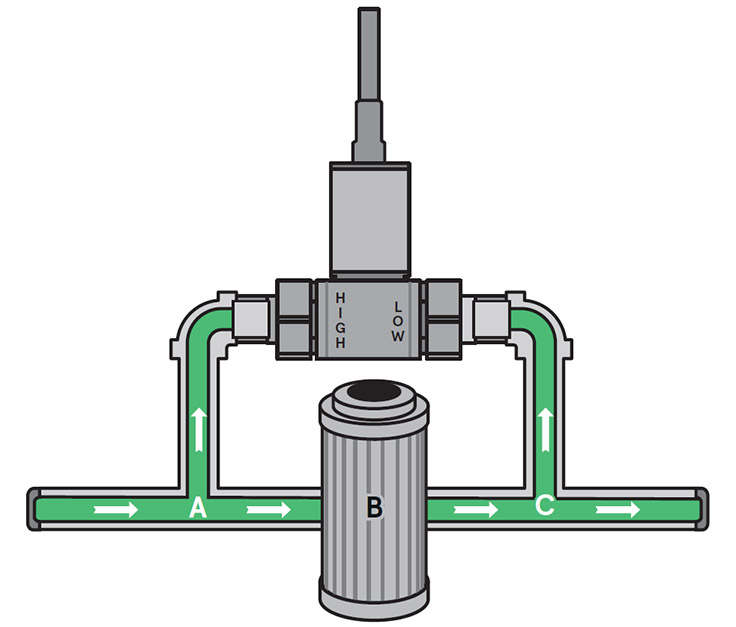
\includegraphics[scale = 0.3]{images/Process-Flow-Pressure-Sensor-EN-Image.jpg}
\label{filtro1}
\caption{Transdutor de pressão diferencial (Fonte: http://www.te.com/usa-en/products/sensors/pressure-sensors/pressure-transducers/differential-pressure-transducers-for-filtration.html)}
\end{figure}

\paragraph{2.  Monitoramento de loops de controle: }

Além de serem usados para monitorar processos, os sensores de pressão geralmente são instrumentais no circuito de controle. Isso é particularmente relevante no uso de hidráulica, onde fluidos pressurizados são usados para aplicar esforço em prensas ou elevadores, por exemplo.

Os sensores geralmente são pequenos, principalmente aqueles baseados na tecnologia MEMS (Sistemas Microeletromecânicos  - \textit{Micro-Electro-Mechanical Systems}, em inglês). Eles podem medir menos de 2 mm em cada lado, mas ser capazes de medir pressões absolutas na região de 20 Bar ou mais. Isso os torna adequados em uma variedade de aplicações, incluindo médica e automotiva.



\subsection{Encoder}

O Encoder  é um dispositivo sensor que fornece \textit{feedback}. Os encoders convertem o movimento em um sinal elétrico que pode ser lido por algum tipo de dispositivo de controle em um sistema de controle de movimento, como um contador ou PLC. O encoder envia um sinal de \textit{feedback} que pode ser usado para determinar a posição, contagem, velocidade ou direção. Com a utilização de encoders, é possível quantizar distâncias, controlar velocidades, medir ângulos, número de rotações, realizar posicionamentos, rotacionar braços robóticos e etc.

O encoder é composto basicamente por um disco com marcações, um componente emissor e um receptor. Os encoder ópticos utilizam LED como o componente emissor e um sensor fotodetector como o receptor.

\begin{figure}[H]
\centering
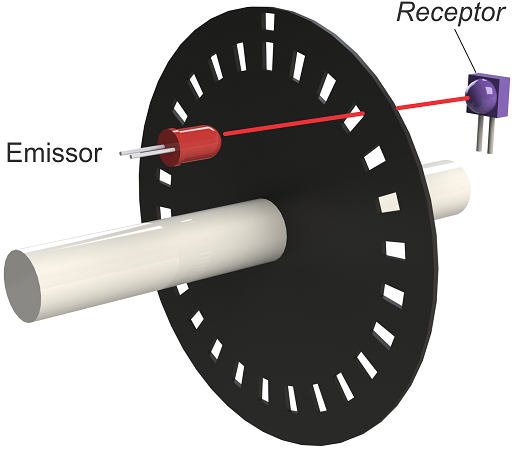
\includegraphics[scale = 0.5]{images/post_encoder3b.png}
\label{filtro1}
\caption{Encoder - emissor e receptor (Fonte: HiTecnologia)}
\end{figure}

As marcações no disco possuem a funcionalidade de bloqueio e desbloqueio do feixe de luz do led para o fotodetector, desse modo,  medida que o disco vai girando o fotodetector juntamente com um circuito eletrônico repassa para as saídas do encoder um sinal em forma de uma onda quadrada, proporcional ao número de marcações do encoder, de acordo com a resolução do mesmo. Logo, a resolução do encoder é o número de marcações presentes no disco do dispositivo, que equivale a quantidade de ondas quadradas, ou clock, gerado em uma volta do encoder.

\begin{figure}[H]
\centering
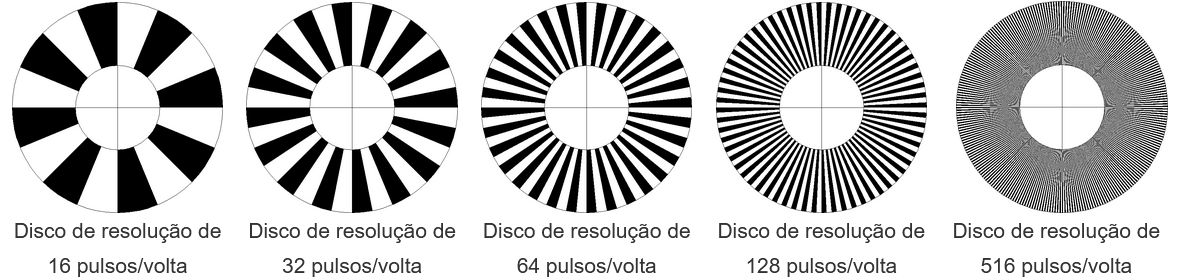
\includegraphics[scale = 0.5]{images/encoders.png}
\label{filtro1}
\caption{Características de marcações dos encoders (Fonte: HiTecnologia)}
\end{figure}

O encoder óptico incremental, o mais comum do mercado, possui 3 sinais de saída: "A", "B" e "O". Com esses sinais adquire-se o ângulo de rotação, o sentido da rotação e o início/fim de uma volta. O sinal A é o sinal principal, que fornece os pulsos (\textit{clock}) a medida que o encoder gira. O sinal B é equivalente ao sinal A, porém defasado em + ou -90°, cujo objetivo é sinalizar o sentido da rotação, e o sinal O (ou Z ou I) indica o início de uma revolução.

\begin{figure}[H]
\centering
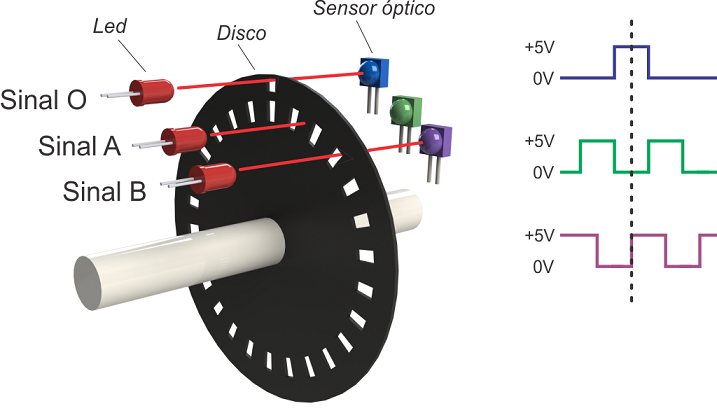
\includegraphics[scale = 0.5]{images/post_encoder3a.png}
\label{filtro1}
\caption{Sinais de saída do encoder}
\end{figure}


Quando o sinal B estiver adiantado em 90º do sinal A, o encoder gira no sentido anti-horário, neste caso a borda de subida de um sinal A se encontra com o sinal B no estado 1, analogamente, quando a B estiver em 0 durante a borda de subida do sinal A, o encoder estará girando no sentido horário.

O terceiro sinal do encoder, o sinal O ou Z ou I, tem por objetivo indicar a posição "0" (zero) do encoder, com essa informação é possível detectar o número de voltas completas que o dispositivo acoplado ao encoder gerou.

\begin{figure}[H]
\centering
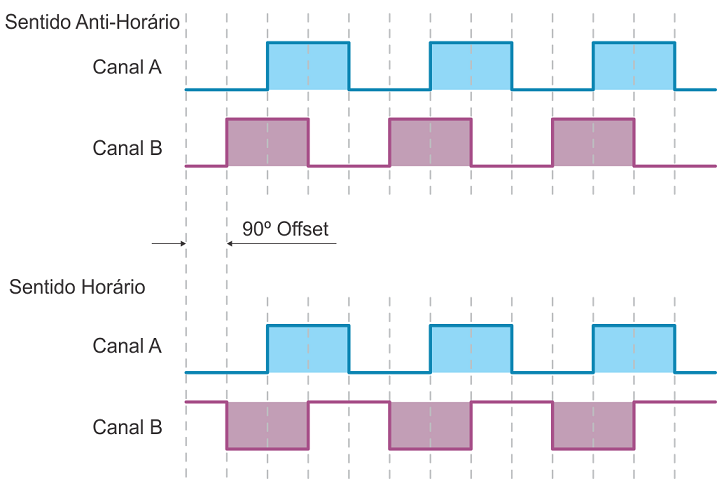
\includegraphics[scale = 0.5]{images/post_enc_04a.png}
\label{filtro1}
\caption{Sinais de saída quanto ao sentido de rotação}
\end{figure}

\subsubsection{Alguns exemplos de aplicação}

Um dispositivo de controle pode usar essas informações para enviar um comando para uma função específica. Por exemplo:

\begin{itemize}
    \item Em uma aplicação de corte no comprimento , um encoder com uma roda de medição informa ao dispositivo de controle quanto material foi alimentado, para que o dispositivo de controle saiba quando cortar.
    \item Em um observatório, os encodercadores informam aos atuadores em que posição um espelho móvel está, fornecendo \textit{feedback} de posicionamento.
    Nos macacos de elevação de vagões ferroviários , o \textit{feedback} do movimento de precisão é fornecido por encoders, de modo que os macacos levantam em uníssono.
    \item Em um sistema de aplicação de servo rótulo de precisão , o sinal do encoder é usado pelo PLC para controlar o tempo e a velocidade de rotação da garrafa.
    \item Em um aplicativo de impressão, o feedback do encoder ativa um cabeçote de impressão para criar uma marca em um local específico.
    \item Com um guindaste grande , os encoders montados no eixo do motor fornecem feedback de posicionamento para que o guindaste saiba quando pegar ou liberar sua carga.
    \item Em uma aplicação em que garrafas ou potes estão sendo enchidos , o feedback informa às máquinas de envase a posição dos recipientes.
    \item Em um elevador, os encoders informam ao controlador quando o elevador atingiu o andar correto, na posição correta. Ou seja, o \textit{feedback} de movimento do encoder para o controlador do elevador garante que as portas do elevador abram no nível do piso. Sem encoders, você pode se encontrar entrando ou saindo de um elevador, em vez de simplesmente sair para um andar nivelado.
    \item Em linhas de montagem automatizadas, os encoders fornecem \textit{feedback} de movimento aos robôs. Em uma linha de montagem automotiva, isso pode significar garantir que os braços de soldagem robóticos tenham as informações corretas para soldar nos locais corretos.
\end{itemize}

Em qualquer aplicação, o processo é o mesmo: uma contagem é gerada pelo encoder e enviada ao controlador, que então envia um sinal para a máquina realizar uma função.

\section{Sensores de som x sensores infravermelho}
Os sensores de som funcionam a partir do princípio da reflexão de ondas sonoras para medir a distancia do dispositivo em relação ao objeto. O sensor dispara ondas ultrasonicas que ao colidirem com o objeto, refletem e são capitadas pelo sensor. Por vez, este tempo entre disparo e capitação determina a distância entre o sensor e o objeto.

\begin{figure}[H]
\centering
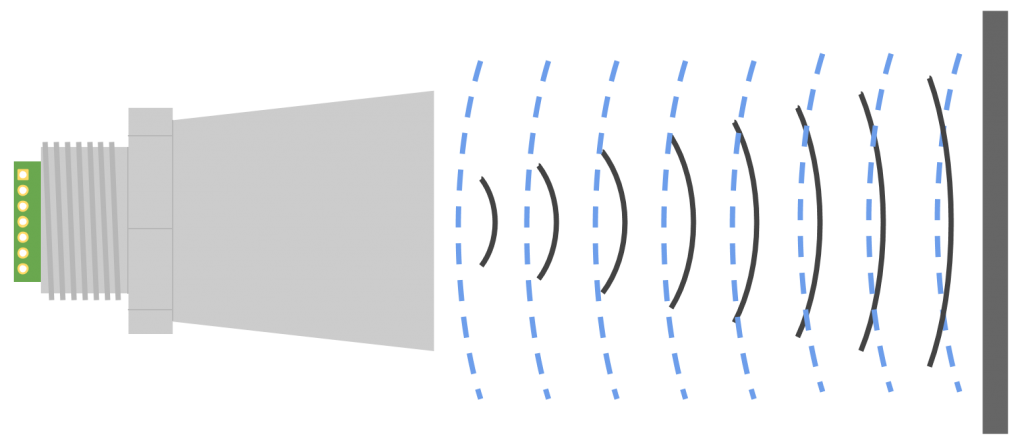
\includegraphics[scale = 0.3]{images/Ultrasonic_sensor.png}
\label{fig:Ultrasonic_sensor}
\caption{Demonstração do funcionamento de um sensor ultrasônico}
\end{figure}

\paragraph{} Os sensores infravemelho por sua vez, utilizam ondas eletromagnéticas(infravermelho) e podem ter a configuração de detecção por reflexão ou por interrupção. Para o primeiro, realiza o mesmo princípio dos sensores de som, a luz infravermelha é disparada e refletida no objeto, e em seguida capitada pelo receptor do sensor, estimando sua distância em relação ao objeto. Já por interrupção, o emissor de sinal e receptor estam alinhados na mesma direção, ativando apenas quando o sinal é interrompido.

\begin{figure}[H]
\centering
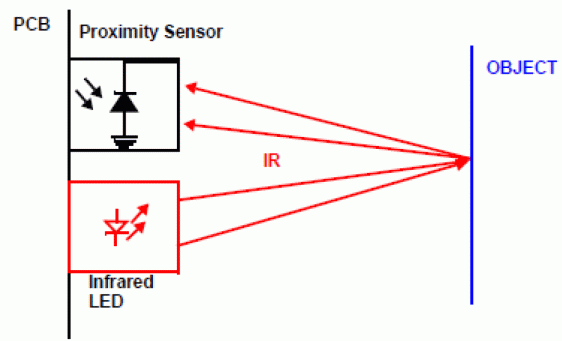
\includegraphics[scale = 0.7]{images/IR_sensor.png}
\label{fig:IR_sensor}
\caption{Demonstração do funcionamento de um sensor infravermelho}
\end{figure}

\subsection{Exemplos de Aplicação}
As aplicações dos sensores ultrassônicos variam imensamente, da construção de um robô para garantir a qualidade de um produto na industria alimentícia. São frequentemente usados em robôs móveis para evitar objetos. Com a finalidade de otimizar o caminho do robô para que não choque com obstáculos, estes sensores são colocados para fornecer a distância exata entre cada obstáculo ao robô. 

\paragraph{}Já na industria, o sensores são utilizados para:
\begin{itemize}

    \item Detectar objetos: Com o sensor, é possível monitorar o preenchimento das embalagens de forma precisa na indústria de alimentos, garantindo que a quantidade correta;
    
    \item Monitorar o nível de preenchimento: Checagem do nível de itens a granel (como grãos) em recipientes (ou mesmo itens líquidos ou sólidos em recipientes estreitos);
    
\end{itemize}

\paragraph{} Os sensores infravermelhos também possuem diversas aplicações, estas sendo em movimentação, comparação ou até como leitores. Algumas dessas configurações são:
\begin{itemize}

    \item Detectores piroelétricos: Sensores com opção de ajustes do gap de operação das ondas sendo utilizado comumente em detectores de incêndio;
    
    \item Detectores de duas cores: Sensor com duplo chip sendo um foto diodo que transmite irradiação infravermelha e um detector de infravermelho, dessa forma é possível captar ondas de diversas frequências, utilizados em medidores de espessura de filme;
    
    \item Detectores foto condutivos: Usam a variação de condutividade dos materiais para incidir radiação, com isso operam com diversas características de frequência e velocidade, aplicados geralmente em imagem térmica;
    
\end{itemize}

\subsection{Vantagens e Desvantagens}

Os dois tipos de sensores possuem diversas aplicações, como apresentado anteriormente. Porém, analisaram-se suas vantagens e desvantagens com respeito a medição de distância. Como foi informado, o sensor ultrasônico opera com ondas sonoras, fazendo com que interferências externas não afetem a performance do dispositivo. Diferente no caso do sensor infravermelho, onde luz, poeira, fumaça e vapor podem interferir na medição. 

\paragraph{}Dependendo da aplicação, o uso do infravermelho é mais vantajoso, já que no mercado é mais barato que um ultrasônico. Se o projeto necessecita de apenas detectar um objeto em sua frente, sem se preocupar com a exata distância, o infravermelho é uma opção viável. Mas se a  medição da distância tem que ser precisa, o sensor ultrasônico se torna a melhor opção.




\section{Referências}
%\bibliography{sample.bib}{}
%\bibliographystyle{ieeetr}
%\bibliographystyle{ieeetr}
%\bibliographystyle{unsrt}
%\bibliography{example}
\printbibliography
%\printbibliography %Prints bibliography
\end{document}